\chapter{Supernova cosmology, et cetera} \label{ch:standard_candles}

We want to use the relationship between the apparent brightness and the known (or calibrated) luminosity of objects to measure the cosmological model through the luminosity distance $D_L(z)$, ultimately depending on the expansion history $a(t)$.  Type Ia supernovae are luminous and fairly consistent explosions of white dwarf stars and have been the workhorses for cosmological measurements of this type.  They are complicated objects, not understood from first priciples, but are well-characterized and standardized.  They are luminous enough and common enough to be seen in large numbers well into the Hubble flow.

In the following, we will describe the supernovae and the Cepheid variable-type stars used to calibrate their luminosities.  We will examine in detail how to properly measure  photometry and spectra in an expanding universe.  These are the necessary data.  Then we will see how researchers build a statistical model of the Type Ia spectral energy distribution and, finally, how this used to make a calibrated distance estimate for each object.

At the end, we'll also discuss some alternative objects and methods for measuring distance, including other types of supernovae and stars, and even gravitational waves.  The statistical methods to fit a cosmological model to these distance measurements are discussed in chapter \ref{ch:likelihoods_cosmology}.


\section{Distance ladder}
Although many Type Ia supernova have been studied in detail with photometric time series of their brightness---so-called ``light curves''---in multiple spectral bands---and a smaller subset have had more-costly spectroscopic measurements to characterize their full spectral energy distributions, that information cannot on its own tell us how luminous the explosions are.  None are close enough for a direct geometric measurement of their distance.  We need to calibrate them with another type of object, usually Cepheid variable stars.  Some Cepheids are near enough to us to measure their distance geometrically via parallax, using the Earth's orbit around the Sun, the size of which is precisely known from radar ranging to the planets.  We know those Cepheids' luminosities by comparing their measured brightness to that distance.  By extrapolating those results to Cepheids that are too far for parallax but bright enough to see in intermediate-distance galaxies that also hosted Type Ia supernovae, we can determine the distances to those galaxies and calibrate the luminosities of the Type Ia supernovae as a class.

% Using nomeclature of 2025arXiv251023823H
Thus to build a ``ladder'' to the distant Universe, we use parallax measurements (rung 1) of the Milky Way Cepheids to anchor the luminosity calibration for the Cepheids.  Then we use extragalactic Cepheid brightnesses (rung 2) as a primary distance indicator to determine distances to the galactic hosts of supernovae and calibrate their luminosities.  We then use the supernovae as secondary distance indicators \citep[rung 3,][]{2025arXiv251023823H}.  We explore some alternative rungs at the end of the chapter.

The next two subsections explain what Type Ia supernova and Cepheid variable stars actually are.  Skip those sections if you just want to know how to use them for cosmology.


\subsection{Type Ia supernova} % What is a SNIa?

\begin{figure}
  \begin{center}
        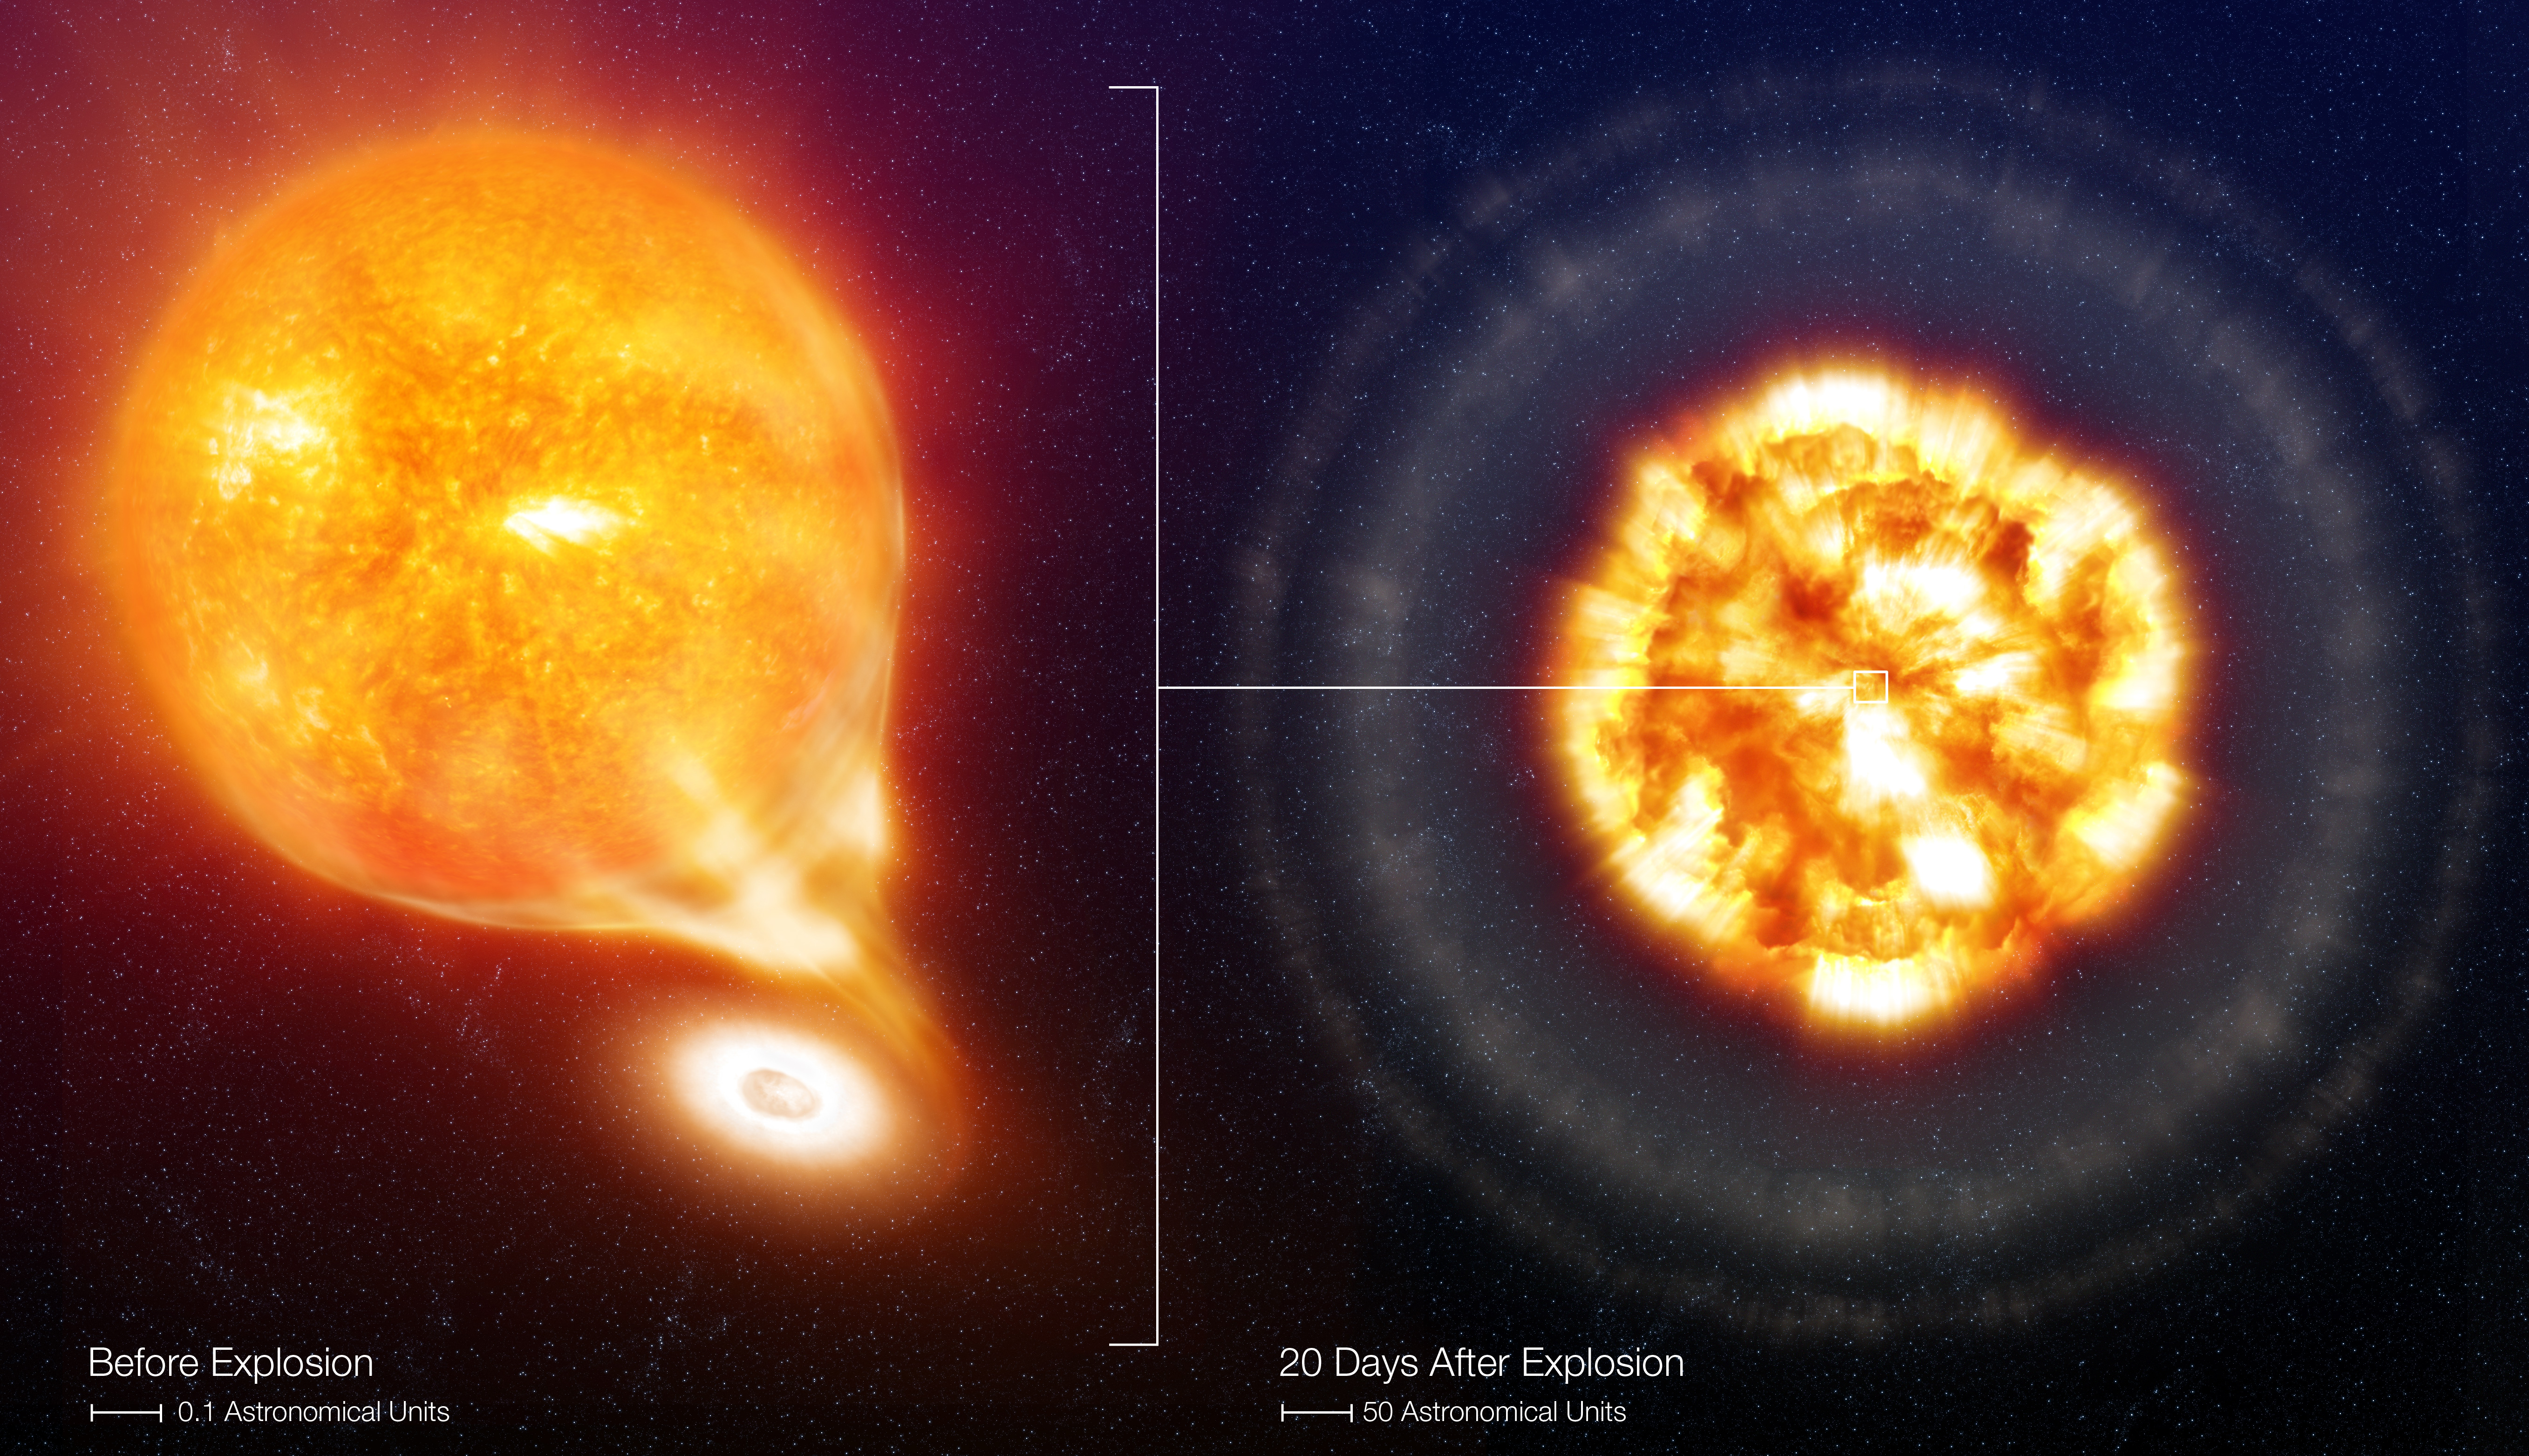
\includegraphics[height=4.3cm]{figs/standard_candles/SN_2006X,_before_and_after_the_Type_Ia_Supernova_explosion_(artist's_impression).jpg}
\hfill
    \includegraphics[height=4.3cm]{figs/standard_candles/SN_1006.jpg} % https://commons.wikimedia.org/wiki/File:SN_1006.jpg
  \end{center}
\caption{Left and center:  before a Type Ia explosion, in an artist impression of the single-degenerate scenario, an evolved giant star donates material to the small white dwarf, eventually triggering an explosion.  After $\sim 20--30 days$, the photosphere of the reaches its maximum luminosity.  Right: the nearly-spherical remnant of historical SN 1006, 1000 years after the explosion, seen by Chandra telescope in three bands of x-rays and thought to be a Type Ia supernova in the Milky Way galaxy.  The diameter is about 19 pc or 4.0 million AU.  There is no clear candidate for the companion, so this supernova may have formed in a double-degenerate (two-white-dwarf) collision that was completely disrupted.}
\end{figure}

A Type Ia supernova is the catastrophic nuclear explosion of a white dwarf star.  White dwarfs are the evolutionary endpoint for the cores of low-to-medium mass stars, under about $8\ M_\odot$.  Most of these stars are composed of carbon and oxygen, having burnt hydrogen to helium during their main sequence lifetimes.  They proceeded to swell up transiently as red giants, and then burnt their core helium to carbon and oxygen as a horizontal branch star.  After swelling again to form asymptotic giant branch stars, the stars shed the outer layers to leave the bare cores, the white dwarf.

A typical white dwarf is similar in size to the Earth (radius $\sim 6000$ km) but contains $\sim 1$~$M_\odot$ of material, yielding a density $\sim 10^9$ kg/m$^3$.  Counterintuitively, the more massive white dwarfs are smaller, compacted by their strong gravity to higher density.  The core of a white dwarf is not fusing, and rather than being supported by the gas pressure due to its temperature, as in a normal star, it is supported by the degeneracy pressure of the dense electrons which, following the Pauli exclusion principle, pile up to fill all the lowest energy states up to the Fermi level.

White dwarf stars have a maximum mass, about 1.4 $M_\odot$ for a non-rotating star, the Chandrasekhar limit\index{Chandrasekhar limit}.  Above that, electrons even in the lowest available energy states become relativistic, provide a softened equation of state, and are unable to support the core against collapse.  Before the core reaches that point, however, the increasing density triggers a thermonuclear detonation of the carbon fuel, powering the explosion.  This is the difference between the carbon-oxygen white dwarf's thermonuclear supernova and the core-collapse supernova of a higher-mass star, where the core has already burned to iron and there are no more exothermic fusion reactions once the electron pressure gives out.  The thermonuclear explosion disrupts the white dwarf, typically leaving no compact remnant,\footnote{An exception is the rare subtype Iax, where the supernova leaves behind a fragment of the white dwarf, known as a zombie star.} while a core-collapse supernova will leave behind a neutron star or black hole.

Where does the white dwarf get the extra mass to explode?  There are two main pathways.  In the single-degenerate-progenitor model, the star starts in a binary system of two main sequence stars.  The more massive, primary star evolves quicker and forms a giant star first, temporarily enveloping the secondary star (a process that ejects mass and angular momentum and reduces the orbital distance between the stars), then proceeds to form the white dwarf star.  Later, the second star evolves and swells into a giant, allowing the primary white dwarf to capture and accrete the tenuously-held outer layers.  A white dwarf that explodes with this mechanism will always be smaller than the Chandrasekhar mass.  These account for perhaps fewer than 20\% of Type Ia supernovae.

In the double-degenerate-progenitor model, the explosion comes from two white dwarfs colliding.  This could happen in a dense star cluster, or in a binary system disrupted by the close passage of a third star or another binary system; the collision of isolated stars is possible but too rare to account for the Type Ia rate.  A close binary of white dwarf stars will have its orbit decay via gravitational radiation.  Once the stars merge, the mass before the imminent explosion may exceed the Chandrasekhar limit.  The double degenerate scenario is favored for most Type Ia supernova because of the lack of suitable companion stars in Type Ia supernova remnants, and because of the lack of observed X-ray emission in active supernovae, which would result from the interaction of the explosion and a companion's outer layers.  The numbers of observed binary white dwarfs are also in line with the observed rate of Type Ia supernova, about  $0.55^{+0.50}_{-0.29}$ (stat.) $\pm 0.20$ (sys.) Mpc$^{-3}$ year$^{-1}$ \citep[][]{2015A&A...584A..62C}, or about 1 supernova per century in a Milky Way-sized galaxy. This is not too hard to find regularly in a survey that covers sufficient volume: look repeatedly at 100 such galaxies and you'll find one each year. You can scale up from there.

\begin{figure}[!t]
  \begin{center}
    \includegraphics[width=0.49\textwidth]{figs/standard_candles/SNIacurva.png} % https://commons.wikimedia.org/wiki/File:SNIacurva.png
    \includegraphics[width=0.5\textwidth]{figs/standard_candles/stretch_correction.jpg} % Figure 1 from 2003PhT....56d..53P
  \end{center}
\caption{Left: Light curve of a type Ia supernova, the initial peak powered by radioactive nickel, followed by a long tail of emission from radioactive cobalt which has a longer half-life.  Right: stretch-correcting the light curve and peak luminosity \citep[from][]{2003PhT....56d..53P}.} \label{fig:Ia_light_curve}
\end{figure}

The exact explosion mechanism inside the white dwarf is an area of active research. As the nuclear burning front moves through the star, it could be subsonic (a deflagration) or supersonic (a detonation).  A pure deflagration model is disfavored because the slower burning allows the star to expand and adjust to the changing temperature and pressure, resulting in a less luminous explosion and paucity of burned products. A pure, supersonic detonation is also disfavored because it traverses the star before the star can react hydrodynamical, and yields a near totally complete burning of the carbon-oxygen fuel to iron group elements (iron, nickel, and cobalt).

The currently-favored model is in-between.  It starts with a deflagration that expands and mixes the star slightly, followed by a detonation, which yields the appropriate amount of intermediate mass elements (like silicon, sulfur, and calcium) and iron group elements.  Another model experiences a detonation in an exterior shell of helium that sends a shock wave into the interior, triggering the main detonation deep inside.  Different mechanisms may be at play in different explosions.  The energy released within a few seconds by the nuclear fusion is sufficient to unbind the star.


Matter is ejected in an expanding shockwave at 5,000--20,000 km/s.  As the density of the outer layer falls, the photosphere become optically thin, successively revealing interior layers with different compositions and yielding a complex spectral behavior.  The explosion creates radioactive $^{56}$Ni in abundance.  With a 6.1 day halflife, this beta decays to $^{56}$Co. The peak luminosity and susequent fading from the peak is powered by this radioactive nickel (Figure~\ref{fig:Ia_light_curve}).  The resulting $^{56}$Co beta decays to stable $^{56}$Fe with a 77.2 day halflife.

The more $^{56}$Ni produced, the more luminous the supernova.  Empirically, the more luminous light curves\index{light curve}---time-series of photometric brightnesses---are broader; they take more time to peak and decline (also Figure \ref{fig:Ia_light_curve}).  Supernova with greater nickel abundance have higher temperature and more highly ionized gas, which leads to higher opacity and a longer photon-diffusion timescale, so they glow for more time.  As iron group ions recombine, they produce overlapping absorption lines, particularly in the UV and blue end of the spectrum.  The hotter, more luminous supernova (with more $^{56}$Ni), where this recombination is delayed, tend to be bluer, and decline slower in the blue B band where the analysis is typically normalized.

Spectroscopy takes more time on a telescope than photometry, and ``Type Ia'' was originally an observational, spectral classification.  Because the progenitor is a carbon-oxygen-rich object, having shed the outer layers, the supernova shows no hydrogen lines, making it a Type I supernova instead of a Type II with hydrogen.  Type Ia spectra show an absorption feature from silicon, one of the intermediate-mass fusion products, while the other classes of Type I supernovae, Ib and Ic, lack this line.   (These are core-collapse supernova of more massive stars that have shed their hydrogen or both hydrogen and helium layers before exploding.  Accordingly, Type Ib include helium lines and Type Ic lack them.)  Type Ia  supernovae can also be distinguished by photometry alone, from their unique nickel-to-cobalt-shaped light curves.


At the date of this writing, the most distant Type Ia supernova is at redshift $z=2.9$, seen in the first two years of JWST data \citep[SN 2023adsy,][]{2025A&A...701A..70V}, although this will likely be surpassed soon.  The total number of well-measured Type Ia supernovae that are included in cosmological analysis is somewhat less that \textcolor{red}{2000}.  These require multiband light curves to characterize the maximum brightness and estimate the main corrections to the luminosity, the light curve timescale and the supernova color.  The number of supernovae with Cepheid-calibrated distances, and thus some notion of their intrinsic luminosity, is not large, perhaps under \textcolor{red}{70}.


  
\section{Point sources of radiation}

We can characterize the brightness of an object by its spectral flux density, which tells you how much energy per time you would collect from that source in unit collecting area within a unit bandwidth of the radiation spectrum.  
%Looking at the definition of flux density and its units, it is clear that
In order to figure out how much energy $E$ you would receive from an object during an observation, you need to integrate the flux density $f_\lambda$ over the time of observation $dt$, collecting area $dA$, and bandwidth $d\lambda$.
\begin{equation}
  E = \int f_\lambda \, dt\, dA\, d\lambda
\end{equation}
The units for brightness, or flux density, are thus $\mbox{W m}^{-2}\mbox{ m}^{-1}$ where the  m$^{-2}$ corresponds to area and the $m^{-1}$ corresponds to wavelength.
If the detectors are not equally efficient at every wavelength or over all parts of the receiver's collecting area, in practice you need to multiply the flux density by efficiency factors that are a function of wavelength (or position) before integrating, such as
\begin{equation}
  E_{\rm band} = \int R_{\rm band}(\lambda) f_\lambda \, dt\, dA\, d\lambda
\end{equation}
where $R_{\rm band}(\lambda$) is the efficiency of the detector/filter combination, which ranges from zero to one.
Here we have assumed that we are describing the spectrum in terms of the wavelength  $\lambda$ of the radiation (common in optical astronomy), but this could equivalently be done in terms of the frequency $\nu$ of radiation (common in radio astronomy).  If we think of
\begin{equation}
   f_\lambda = \frac{dE}{dt \, dA \, d\lambda}
\end{equation}
as we have done above, or alternatively,
\begin{equation}
  f_\nu = \frac{dE}{dt \, dA \, d\nu}
\end{equation}
then it becomes clear that
\begin{equation}
  f_\nu = f_\lambda \left| \frac{d\lambda}{d\nu} \right| = f_\lambda \frac{c}{\nu^2} = f_\lambda \frac{\lambda^2}{c}
\end{equation}
where we have used the speed of light and the relation $\lambda = c/\nu$ in the last equations.  Even though $\lambda$ decreases when $\nu$ increases, so the derivative is negative, by convention we make both spectra $f_\nu$ and  $f_\lambda$ positive, which accounts for the absolute value.

We don't receive much power from astronomical objects.  In radio, microwave, and sub-millimeter band astronomy, the typical unit for brightness is called the Jansky, which in SI units is
\begin{equation}
  1\ \mbox{Jy} = 10^{-26}\ \mbox{W m}^{-2}\mbox{ Hz}^{-1}.
\end{equation}


We can model the contribution of a point source to the surface brightness sky signal as a delta function:
\begin{equation}
  s_\lambda(\hat n) = f_\lambda \delta( \hat n - \hat n_0)
\end{equation}
where $\hat n$ is a direction on the sky and $\hat n_0$ is the vector that points to the source of radiation.  If we thus integrate any area of sky (or \textit{aperture}) that contains the source, we get the value $f$ of its brightness. Note that the delta function  on the two-dimensional sky has units of inverse angle squared, or inverse solid angle. 

Of course, telescopes do not have perfectly sharp imaging, and so radiation coming from one direction is detected from other, nearby directions.   Light from a single direction spreads out onto the focal plane, falling into several pixels on the camera.  This effect of the telescope's resolution we call the ``point-spread function'' in optical or infrared astronomy, because it describes how a point of light is spread out on the image. In radio and microwave astronomy, we call the same thing the telescope ``beam,'' because if you reverse the purpose of the radio dish, and use it as a transmitter instead of a receiver, the point-spread function describes intensity of the beam of radiation that the horn or dish puts out as a function of angle to the telescope boresight.  The original delta function of radiation gets convolved to produce the image of surface brightness captured by our camera exposure.

We will continue a detailed discussion of the point spread function or beam in Chapter \ref{ch:CMB} on the cosmic microwave background, where it figures into an important correction for the measurement of fluctuations.  For now we will assume that we can get good photometry, a good measurement of the brightness, by integrating up the light from the star or supernova as it is spread by the optics across several camera pixels.

The bolometric brightness of an object, which occurs in the definition of luminosity distance (Equation \ref{eqn:DL}), is
\begin{equation}
  F = \int_{{\rm all}\ \lambda} f_\lambda d\lambda 
\end{equation}
or
\begin{equation}
f_\lambda = \frac{dF}{d\lambda}
\end{equation}
while the flux in a band, is
\begin{equation}
  F_{\rm band} = \int R(\lambda) f_\lambda d\lambda = \int R(\lambda) s_\lambda d\lambda d\Omega. \label{eqn:flux_in_band}
\end{equation}
using the band filter function $R(\lambda)$. It is straightforward to make similar expressions employing $f_\nu$.

The band-averaged flux density is
\begin{equation}
  f_{\rm band} = \frac{\int R(\lambda)  f_\lambda d\lambda}{\int R(\lambda) d\lambda} = \frac{F_{\rm band}}{\int R(\lambda) d\lambda} 
\end{equation}
which is just a weighted average of $f_\lambda$ over the band.  This has the advantage of giving roughly the same value if the band is not too wide compared to features in the spectrum and will give similar values for moderate differences in the band.  You can also think of the effective wavelength of the band for a particular spectrum of source
\begin{equation}
  \lambda_{\rm band} = \frac{\int \lambda R(\lambda)  f_\lambda d\lambda}{\int R(\lambda)  f_\lambda d\lambda} = \frac{\int \lambda R(\lambda)  f_\lambda d\lambda}{F_{\rm band}}
\end{equation}
which is like the mean wavelength or a first moment of the spectral/band distribution.  Unless that distribution is multimodal (multiple peaks), this will be the wavelength near where the flux density equals the band-averaged flux density.

\begin{figure}
  \begin{center}
    \includegraphics[width=0.7\textwidth]{figs/standard_candles/photometric_systems.png}
  \end{center}
  \caption{Filter functions of some photometric systems, with wavelength measured in angstroms ($= 0.1$ nm) along the x-axis.  The letters or numbers give an indication of the color or effective wavelength.
    Adapted from \citep{2005ARA&A..43..293B}} \label{fig:photometric_systems}
\end{figure}

Every telescope has its own filters and wavelength response that define its bands.  Some notable photometric systems include the Johnson UBV system, Rubin-LSST ugrizy, and SDSS u',g',r',i',z'.  Usually U/u means ultraviolet, B means blue, V means visible, g means green, R/r means red, I/i means infrared, and other letters (J,K,z) mean farther in the infrared.  (See Figure \ref{fig:photometric_systems} for some examples.)  Hubble Space Telescope's WFC3 and James Webb Space Telescope's NIRCam have filters named for their central wavelength and shape, for example NIRCam's F150W, a  band centered at 1.5 $\mu$m that is 0.4 $\mu$m ``wide,'' wider than the other bands at the same wavelength.


\subsection{Magnitude system}
I am no great fan of it, but it is common in astronomy to use the traditional 19th-century logarithmic system of \textbf{stellar magnitudes}\index{magnitude system} to describe the brightness of objects.  Magnitude systems have two properties.  First, if two fluxes are in a ratio of 100, they will differ by 5 magnitudes, with the brighter having the \textit{lower} magnitude.\footnote{This connects back to the 2000-year-old visual star catalog of Greek astronomer Hipparchus (and popularized by Ptolemy) who ranked the brightest stars as first magnitude, the next brightest as second magnitude and so on.}  The second property sets the zero point for the magnitude scale and warrants more discussion below.

The relationship between fluxes and magnitudes is thus
\begin{equation}
  \frac{F_1}{F_2} = 100^{(m_1-m_2)/5},
\end{equation}
or equivalently,
\begin{equation}
  m_1-m_2 =  -\frac{5}{2} \log_{10} \left( \frac{F_1}{F_2} \right).
\end{equation}
Here $m_1$ and $m_2$ are called apparent magnitudes because they are based on the brightness that is apparent to our observation.

Although the magnitude carries the same information as the flux, and perhaps adds some unnecessary confusion, the magnitude system does ease the job of calibrating the photometry in the following sense.  It is straightforward to get relative calibration for a target object by comparing the ratio of its brightnesses to a calibration star in the same image with a known magnitude.  Any multiplicative calibration factors inherent to that particular image divide out, like the time of exposure or efficiency of the detector.  If no calibration star is available, the magnitude calibration can be chained back, bright star to bright star, to one of known brightness though several links.  For calibration, it's only straightforward to compare two fluxes of alike types, for example, two bolometric fluxes or two g-band fluxes.

There are two common choices of normalization or zero point, stellar-based or absolute.  The normalization can be thought of as choosing a reference flux in the band
\begin{equation}
  m_{\rm band} = -2.5 \log_{10} \left( \frac{ F_{\rm band}}{F_{{\rm ref},\ \rm band}} \right) = -2.5 \log_{10} \left( \frac{ f_{\rm band}}{f_{{\rm ref},\ \rm band}} \right) ,
  \label{eqn:reference_flux}
\end{equation}
(equal because the band-averaged $f$s have denominators that cancel) or equivalently an additive constant in
\begin{equation}
  m_{\rm band} = -2.5 \log_{10} \left( \frac{ F_{\rm band}}{[\mbox{flux unit}]} \right)  + C_{\rm band}.
\end{equation}
The Vega magnitude system chooses these references so that the magnitude of the star Vega is zero in all bands, using $F_{{\rm ref},\ \rm band} = F_{{\rm Vega},\ \rm band}$.  Vega, a spectral type A0 star with blackbody temperature about 8,900 K, is a slightly problematic choice for precision work since it is variable by about a tenth of a magnitude.  The similar Johnson UVB system defines zero magnitude in each band with the average of six stars with the same spectral type as Vega.

The AB magnitude system, on the other hand, provides an absolute energy calibration without depending on particular stars.
For any bandpass filter, it is defined so that
\begin{eqnarray}
  m_{AB} &=& -2.5 \log_{10} \left( \frac{\int R(\nu) f_\nu d\nu}{\int R(\nu) (1\mbox{ Jy})  d\nu} \right) + 8.90 \\
  &=&  -2.5 \log_{10} \left( \frac{\int R(\nu) f_\nu d\nu}{\int R(\nu) (1\mbox{ erg s}^{-1}\mbox{ cm}^{-2}\mbox{ Hz}^{-1}) d\nu}  \right) - 48.60, \nonumber
\end{eqnarray}
or
using a reference flux in equation \ref{eqn:reference_flux} of
\begin{equation}
  F_{{\rm ref,\ band}} = \int R(\nu) (1 \mbox{ Jy} \cdot 10^{-8.90/-2.5}) d\nu \approx \int R(\nu) (3631 \mbox{ Jy}) d\nu.
\end{equation}
Note that $f_\nu = 3631$ Jy is close to the flux density of Vega in V band (but not other bands) and is the reason that value was chosen.  AB magnitudes make a pretty good definition because it puts the scale on firm footing with respect to energy units.\footnote{Note that these expressions are sometimes written for a very narrow filter over which the $f_\nu$ doesn't vary, and the integral $\int R(\nu) d\nu$ is canceled on top and bottom, leaving only e.g.\ the $(f_\nu/1\mbox{ Jy})$ in the logarithm and defining a monochromatic magnitude rather than a band magnitude.  Sometimes the units are left out of the equation entirely, but mentioned in text instead, which I think is a confusing abuse of unit notation.  Other times, the filter function is written as $R(\nu) =  p(\nu) (h\nu)^{-1}$ where $p(\nu)$ is the ``capture cross section'' that quantifies the probability of counting an incident photon as an $e^-$ in the detector.  The $h\nu$ is the energy of that photon to convert between the fraction of photons getting through and the fraction of energy getting through.  It helps to pay careful attention to these definitions when you encounter a bandpass function.}
To actually measure $m_{AB}$ from an image, you still have to go through a chain of calibration, typically using standard stars along the way.

A \textbf{color index}\index{color index} difference between the magnitudes in two bands, like $m_B-m_V$ (often written a simply $B-V$), is a comparison of the received energy flux between the bands.  In a Vega-based magnitude system, it is the base-10-logarithm of that ratio divided by the similar ratio from Vega.  Thus stars with the same spectrum as Vega have color indices equal to zero for all pairs of bands.  Across the visual bands, for smaller wavelength magnitudes minus larger wavelength magnitudes, the color index is negative for stars hotter than Vega and positive for stars cooler than Vega.

One disadvantage of the magnitude system is that it becomes difficult to add or accumulate.  
Two 10.0 magnitude stars in binary system add to a total magnitude of 9.25 while two 20.0 mag stars add to a total of 19.25 because the decrease $\Delta m = -0.75$ corresponds to a doubling
of flux.
The common practice of providing surface brightness with a unit of mag/arcsec$^2$ is really terrible.  It means that a 1 arcsec$^2$ pixel would have a flux corresponding to the particular magnitude (regardless of the actual pixel size), but these must be converted back to flux to add it up.

For supernova cosmology analysis, it is important to bring all the varied photometry of various supernova over the year to a common photometric system, which entails a multitude of telescopes and filters with secondary and tertiary stars common between various surveys needing to be compared and modeled \citep[e.g.][]{2022ApJ...938..111B}.  Such reliable photometry is vitally important and a lot of work.

The dust in the Milky Way alters the spectrum of any extragalactic object we see, attenuating the blue light and reddening the color.  This is typically written as $E(B-V)$, which actually means $(m_B - m_V)(\hat \mathbf{n})$, the magnitude difference due to dust reddining as a function of position on the sky.  This has been tabulated by measurements  of the dust column density either through long-wavelength observations of the dust emission or via spectral features of the dust.

\subsection{Distance modulus}
While the apparent magnitude measures the brightness of an object, the \textbf{absolute magnitude}\index{absolute magnitude} measures its luminosity.  The absolute magnitude $M$ is defined as what the apparent magnitude would be if we imagine the object were 10 pc away.\footnote{Absolute magnitude was conceived for stars and is kind of inappropriate for a supernova, since a supernova at 10 pc would be exceedingly dangerous, destroying the ozone layer and causing a mass extinction on Earth.}  Considering bolometric magnitudes, 
\begin{equation}
  100^{(m_{\rm bolo}-M_{\rm bolo})/5} = \frac{F_{10\ \rm pc}}{F} = \frac{{L}/{4\pi(10\ \rm pc)^2}}{{L}/{4\pi D_L^2}} = \left( \frac{D_L}{10\ \rm pc} \right)^2
\end{equation}

The apparent magntitude we can measure and so it is easier to get than the distance or absolute magnitude.  In cosmology, we are often trying to learn the absolute magnitude or the luminosity in order to determine the luminosity distance as a function of redshift and thus the cosmology.


\begin{figure}[!t]
  \begin{center}
    \includegraphics[width=\textwidth]{figs/standard_candles/distance_modulus_of_z.pdf} \\
    \includegraphics[width=\textwidth]{figs/standard_candles/distance_modulus_diff_of_z.pdf}
  \end{center}
  \caption{Distance modulus versus redshift.  The data currently supports models similar to the $\Lambda$CDM one; the others have been ruled out for two decades are are only shown for comparison.  As a point of comparison for distinguishing models, a difference of $\Delta m = 0.1$ magnitudes coresponds to a flux change $\Delta F/F$ of about 10 percent.  A difference of $\Delta m = 0.01$ corresponds to $\Delta F/F$ of about 1 percent.  To measure the distance modulus to that precision, both the measured brightness and the understanding of the intrisic luminosity need to beat that level.}\label{fig:distance_modulus_theory}
  \end{figure}
  
\begin{figure}[!t]
  \begin{center}
    \includegraphics[width=\textwidth]{figs/standard_candles/brout_2022_pantheon_cosmo_hd_wsh0es.png}
  \end{center}
  \caption{Distance modulus versus redshift from \citet{2022ApJ...938..110B} with the Pantheon+ compilation of type Ia supernovae.  Each colored mark indicates the distance modulus of a single supernova light curve measurement and modeling; the colors denote the various surveys.  The upper plot shows the modulus and the lower plot shows the difference to their best-fit model.  The error bars on several supernova averaged together (bold black points) are very constraining on the possible cosmology.} \label{fig:distance_modulus_data}
\end{figure}

Taking the logarithm yields the \textbf{distance modulus}, a measurement of luminosity distance that equals the difference between the apparent and absolute magnitude.  

\begin{equation}
  \mu \equiv   5 \log_{10}(D_L / 10\,\mbox{pc}) =  m_{\rm bolo} - M_{\rm bolo}
\end{equation}

In a band, the absolute magnitude is
\begin{eqnarray}
  M_{\rm band} &=& -2.5 \log_{10} \left( \frac{F_{\rm band,\ 10 \ pc}}{F_{\rm ref, \ band}}  \right)  \\
  &=&   -2.5 \log_{10} \left( \frac{ \int R(\lambda) f_{\lambda,\ 10\ \rm pc}\ d\lambda}{F_{\rm ref, \ band}} \right).
\end{eqnarray}
For the Sun, $M_V = +4.83$ while $m_V = -26.7$.  For Type Ia supernova $M_V \sim -19$.


\subsection{K-corrections}
When you measure an object at high reshift in a filter band, relevant here for cosmology, you must make a further correction.  The emission that you receive is redshifted from that which was emitted and the wavelength increment in the bandwidth is also redshifted.  To compute this correction, let's recall that observed wavelength relates to the emitted wavelength as
\begin{equation}
  \lambda = (1+z) \lambda_{\rm em}.
\end{equation}
Then, for the spectral flux density we will have,
\begin{eqnarray}
  f_\lambda = \quad \frac{dF}{d\lambda} &=& \frac{d}{d\lambda} \frac{L}{4\pi D_L^2} \\
  &=& \frac{d}{d ((1+z) \lambda_{\rm em})} \frac{L}{4\pi D_L^2} \\
  &=& \frac{1}{1+z} \frac{dL/d\lambda_{\rm em} |_{\lambda_{\rm em}} }{4\pi D_L^2} \\
  &=& \frac{1}{1+z} \frac{l_{\lambda_{\rm em}} }{4\pi D_L^2} \\
  &=& \frac{1}{1+z} \frac{l_{\lambda/1+z}}{4\pi D_L^2}.
\end{eqnarray}
This important expression for the observed source spectrum deserves some commentary.  Recall that the luminosity distance is already accounting for the redshifting of energy from the bolometric luminosity in the emitting frame, $L$.  To get the spectrum, we need to take its derivative, but it doesn't make sense to take the derivative of the emitting luminosity with respect to the observed wavelength.  So we convert to a derivative with respect to the emitted wavelength, evaluated at the emitted wavelength.  Then we write the derivative of the luminosity, the spectral luminosity density, as $dL/d\lambda_{\rm em} = l_{\lambda_{\rm em}}$, and substitute in the value of the emitted wavelength.

When you integrate the received flux in a band (\ref{eqn:flux_in_band}), you are effectively integrating over a different band in the emitted frame.
\begin{eqnarray}
  F_{\rm band} &=& \int R_{\rm band}(\lambda) \frac{1}{1+z} \frac{l_{\lambda/1+z}}{4\pi D_L^2}  d\lambda \label{eqn:flux_from_redshift} \\
  &=& \int  R_{\rm band}\left((1+z) \lambda_{\rm em} \right)   \frac{l_{\lambda_{\rm em}}}{4\pi D_L^2} d\lambda_{\rm em}
\end{eqnarray}
We can examine the difference between band magnitude and the distance modulus
\begin{eqnarray}
  m_{\rm band} - \mu &=& -2.5 \log_{10} \left(\frac{F_{\rm band}}{F_{\rm ref,\ band}} \right) - 2.5 \log_{10}  \left(\frac{D_L^2}{(10\ {\rm pc})^2} \right) \\
  &=& -2.5 \log_{10} \left(\frac{ \frac{D_L^2}{({\rm 10\ pc})^2} \int R_{\rm band}\left((1+z) \lambda_{\rm em} \right)   \frac{l_{\lambda_{\rm em}}}{4\pi D_L^2} d\lambda_{\rm em}      }{F_{\rm ref,\ band}} \right)  \nonumber
\end{eqnarray}
The luminosity distances cancel, so we can define the flux we would have observed at 10 pc in the emitted frame, but in the redshift-adjusted band ``$z$band,''
\begin{equation}
  F_{z\rm band,\ 10\ pc} =  \int R_{\rm band}\left((1+z) \lambda_{\rm em} \right)   \frac{l_{\lambda_{\rm em}}}{4\pi ({\rm 10\ pc})^2} d\lambda_{\rm em} 
\end{equation}
Then we find that 
\begin{eqnarray}
  m_{\rm band} - \mu = -2.5 \log_{10} \left(\frac{F_{z\rm band,\ 10\ pc}}{F_{\rm ref,\ band}} \right) \label{eqn:m_minus_mu_simple}
\end{eqnarray}
The right side is not quite the absolute magnitude in either the band or the redshifted band because the bands don't match between the object and the reference flux.  We can insert a correction to make them match.
\begin{eqnarray}
  m_{\rm band} - \mu &=& -2.5 \log_{10} \left(\frac{F_{\rm band,\ 10\ pc}}{F_{\rm ref,\ band}}\cdot \frac{F_{z\rm band,\ 10\ pc}}{F_{\rm band,\ 10\ pc}} \right) \\
  &=& -2.5 \log_{10} \left(\frac{F_{\rm band,\ 10\ pc}}{F_{\rm ref,\ band}}  \right)  -2.5 \log_{10} \left( \frac{F_{z\rm band,\ 10\ pc}}{F_{\rm band,\ 10\ pc}} \right) \\
  &=& M_{\rm band}  +K. %-2.5 \log_{10} \left(  \frac{\int R((1+z)\lambda_{\rm em}) l_{\lambda_{\rm em}} d\lambda_{\rm em}}{\int R(\lambda) l_\lambda d\lambda} \right)
\end{eqnarray}
Thus we find that
%\begin{equation}  m_{\rm band} - \mu = M_{\rm band} + K \end{equation} or
\begin{equation}
  \mu  =  (m_{\rm band} - K) - M_{\rm band},
\end{equation}
relating the distance modulus to the observed magnitude with a correction and the absolute magnitude in the same (observed) band.  The 
 $K$-correction is
\begin{equation}
  K = -2.5 \log_{10} \left(  \frac{\int R((1+z)\lambda_{\rm em}) l_{\lambda_{\rm em}} d\lambda_{\rm em}}{\int R(\lambda) l_\lambda d\lambda} \right), \label{eqn:K-correction}
\end{equation}
where we have canceled the $4\pi(10\ {\rm pc})^2$ in the fraction.

Note any of these expresssions (\ref{eqn:flux_from_redshift})--(\ref{eqn:K-correction}) put you in the slightly uncomfortable position of needing to know the spectrum of the object in order to make the correction accurately.  How much of a mistake you might make when you model that spectrum is something that you need to evaluate. 

Although mathematically correct, I find the $K$-correction an awkward way to deal with this correction, because it corrects the data with a model of the unknown source and uses the absolute magnitude of a wavelength range other than what we actually probe in the rest frame.  An alternative approach would have been to re-express Equation (\ref{eqn:m_minus_mu_simple}) as
\begin{eqnarray}
  m_{\rm band} - \mu &=& -2.5 \log_{10} \left(\frac{F_{z\rm band,\ 10\ pc}}{F_{{\rm ref},\ z{\rm band}}}\cdot \frac{F_{{\rm ref},\ z{\rm band}}}{F_{\rm ref,\  band}} \right) \\
   &=& M_{z \rm band} - 2.5 \log_{10} \left( \frac{\int R((1+z)\lambda) f_{\lambda,\ \rm ref}\ d\lambda}{\int R(\lambda) f_{\lambda,\ \rm ref}\ d\lambda} \right) \label{eqn:alternative_to_K_correction}
\end{eqnarray}
In this formulation, we have the apparent magnitude we actually observe ($m_{\rm band}$), the distance measure ($\mu$), the absolute magnitude we actually probe ($M_{z\rm band}$ in its native, emitted frame), and a correction that does not depend on the unknown spectrum of the source, only the known reference.  However, for supernova cosmology, we need to compare and calibrate many supernova at different redshifts, so even in this formulation we would still need a model for the rest frame spectrum of the objects to model the absolute magnitudes in the redshifts bands.

\textcolor{blue}{In the end, it seems to me that it would be better simply to work with the flux directly (\ref{eqn:flux_from_redshift}) or the equivalent band-averaged flux density $f_{\rm band}$. With the redshift, spectral model, and calibrated photometry, you can seek the luminosity distance directly, bypassing the magnitude system and distance modulus altogether.  However, these are the standards in the field right now (and it's not my subfield) so we will continue to use them.}

\section{Measuring distance}
Let's review where we are.  From Eq.~\ref{eqn:flux_from_redshift}, if we know the intrinsic luminosity of an object in a band (or equivalently its absolute magnitude) then we can compare to the observed flux (or apparent magnitude) to get the luminosity distance for that redshift.  The problem is that we usually don't know the the intrinsic luminosity.

\subsection{Temporal SNIa spectrum models}
We have seen how vital it is to have an understanding of the spectral information of the supernova for dealing with redshift corrections to the photometry.  The spectra of Type Ia supernova change in nontrivial ways as the explosion develops.  Therefore, one of the ingredients in a modern SNIa cosmology analysis is a model of the supernova spectrum as a function of time.  As an example, the widely-used SALT2/SALT3 models \citep[Spectral Adaptive Lightcurve Template,][]{2007A&A...466...11G,2021ApJ...923..265K,2023ApJ...951...22J} use a variety of photometric and spectral data to build an empirical spectrum.  
The modeling is kind of complicated but we include it for completeness.

To build the SALT2 model, each supernova $i$ in the training set is compared against a rest-frame spectral template with the following functional form:
\begin{equation}
  f_{\lambda,i}(t) = x_{0,i} \times [ M_0(t,\lambda) + x_{1,i} M_1(t,\lambda) + ... ] \times \exp( c_i C^{\rm color}(\lambda))
\end{equation}
There are several ingredients here.  The $M_k(t,\lambda)$ are a series of spectral shape templates that are common to all supernova in the model (not absolute magnitudes).  The $x_{k,i}$ parameters record the contribution of these components to each supernova.  The template $M_0$ is a dimensionless average spectral sequence as a function of time,  normalized for a supernova at 1 Mpc, {which gives close zero B-band apparent magnitude at maximum light}, $t=0$; {the corresponding $x_0$ is the overall amplitude for a particular supernova's spectrum, recording the overall brightness}.

The template $M_1$ is the dominant correction to the spectral shape among supernova (approximating the effect of a time stretch);  the $x_{1,i}$ parameter is its contribution (relative to $x_{0,i}$) of that correction.  The $M_1$ and higher corrections change the spectral shape, and thus the $K$ correction, but do not change the B-band magnitude.
%\textcolor{red}{Are $M_k(t=0) = 0$ for $k>0$?}
Further corrections $k$ improve the fit, but are not strongly correlated with the peak luminosity and thus have little cosmological impact.\footnote{The next generation SALT model will include a $k=2$ term.}  The $C^{\rm color}(\lambda)$ is the average color correction law and the $c_i$ is the strength of the correction per supernova.  The fiducial SNIa has $x_1 = 0$ and $c = 0$.

None of the functions $M_k(t,\lambda)$ or $C^{\rm color}(\lambda)$ are known at the outset.  The model fits for them.
The $M_k(t,\lambda)$ are continuous functions parameterized as 3rd-order B-splines (piecewise polynomials with continuous second derivatives).  For $M_k$ templates, the model uses 10 parameters along the time axis, covering $-20$ days to $+50$ days around B-band maximum light and doubling the time resolution between maximum light and $+20$ days.  Although spectral resolution required for modeling photometry is modest, $\lambda/\Delta\lambda \sim 100$, spectral comparisons require $\lambda/\Delta\lambda \sim 1000$--$2000$, requiring some few thousand parameters along the wavelength axis (from 2000 to 9200 \AA).
%For $M_1$ the model uses the same time resolution but only 60 parameters along the wavelength axis.  \textcolor{red}{It is not clear what resolution for higher $k$.}
The color correction $C^{\rm color}(\lambda)$ is a 3rd-order polynomial with two of the four parameters free for the global fit and two fixed: it ensures that $C^{\rm color}(\lambda_B) = 0$, so there is little color effect in B band, and that $C^{\rm color}(\lambda_V) = 0.4$, fixing the amount of reddening between B and V bands for $c_i = 1$.  

In recent incarnations, and depending on quality cuts, this model is fit to about 2000 supernova or more, using photometry and spectra as a function of time. Some groups separate the training set of SNe (for fitting the model) from the cosmological set, which helps to avoid overfitting bias, but other groups use the same SNe for both. Together with the global spline parameters in the $M_k$ and $C^{\rm color}$, there are $x_{0,i}, x_{1,i}, c_i$ parameters for each supernova, totaling several thousand parameters in the model.  Observed spectra typically come with significant broadband systematic fluctuation in the spectrum without an overall normalization, so supernova with spectra include additional parameters to recalibrate the spectra as a function of wavelength, $a_{\rm recal}(\lambda)$.  These parameters are also fit with the others.  

The model initializes the $M_0$ and $M_1$ to the mean and first derviative of a previous model, then computes any subsequent components to be orthogonal to the the previous components ({like a Gram-Schmidt procedure}).  The fitting seeks parameters that minimize a total $\chi^2$ that is the sum of a data term and regularization term:
\begin{equation}
  \chi^2_{\rm SALT2} = \chi^2_{\rm data} + \chi^2_{\rm reg}
\end{equation}

Different groups use somewhat different models statistical models.  A simple data $\chi^2$ looks like a sum for each supernova over observational photometric and spectroscopic data points (index $q$), each of which has it's own position on the sky $\hat n_q$, time epoch ($t_q$), and band (band $q$) or wavelength ($\lambda_q$)
\textcolor{black} {
\begin{eqnarray}
  \chi^2_{\rm data} = \sum_{{\rm SN}\ i} && \left[ \sum_{{\rm photo\ pt.}\ q} {\left(m_{iq} - m_{{\rm band}\ q}[f_{\lambda,i} (t_q,x_i,c_i)|\hat n_q,z_i]\right)^2}/{\sigma_{iq}^2} + \right.
    \\ \nonumber
    &&  \ \left. \sum_{{\rm spec.\ pt.}\ q} (f^{\rm obs}_{\lambda_q}(t_q) - a_{\rm recal}(\lambda_q) f_{\lambda_q}(t_q,x_i,c_i|\hat n_q,z_i) )^2/\sigma_{{\rm spec},i}^2    \right].
\end{eqnarray}
This is simply a giant comparison of all the data from all the supernova to the spectral model, tuned by $x_i,c_i$ for each supernova $i$.}  Note that in this expression, the computed magnitudes are $K$-corrected and the spectra are similarly corrected for the observed redshift $z_i$.  The model spectrum is used to compute the corrections.  At this step, the model spectra are also corrected for Milky Way reddening.   


To compute the magnitudes, the spectral models is integrated against each instrument and band's filter transmission curve.  In some cases the filter function depends on the position in the focal plane.  Such fastidious details are essential for precision photometric comparisons.  Modern spectra typically come with proper error bars.  Some older archival spectra did not, so the spectral errors were adjusted by hand so that the photometry and spectra got equal weight in the fit.

The regularization term is quadratic in the templates
\begin{equation}
  \chi^2_{\rm reg} = A \sum_k M_k^\dag D^\dag D M_k, 
\end{equation}
where the \textcolor{red}{derivative matrix $D$ means what???}, and $A$ is a tunable parameter to control its strength.  The regularization term suppresses the degeneracy where two templates run away in opposite directions. 
The regularization term allows convergence but introduces a bias.  Its amplitude was chosen to keep the bias smaller than 0.005 mag in a simulated dataset for all wavelengths, significantly below statistical uncertainties.

The fitting minimizes $\chi^2$ following a Gauss-Newton algorithm that uses the Jacobian of $\chi^2$ with respect to the fitting parameters.  In an iterative sequence, each step requires solving an $N_{\rm par} \times N_{\rm par}$ linear system (the size of the Jacobian) which provides an update to the parameters.  The fitting iterates until the total $\chi^2_{\rm SALT2}$ stops improving.

\subsection{Distance estimates}
The Pantheon+ catalog for instance uses the following estimator for the distance modulus \citep{1998A&A...331..815T}:
\begin{equation}
  \mu_i = m_{B,i} - M_{B,i}, 
\end{equation}
For each supernova, the apparent magnitude
\begin{equation}
m_{B,i} = -2.5 \log_{10} \left(x_{0,i} \times \frac{\int d\lambda R_{\rm B}(\lambda)\, M_0(t=0,\lambda)}{F_{{\rm ref},B}} \right) \approx -2.5 \log_{10} (x_{0,i})
\end{equation}
comes from that supernova's fit to the SALT model and is the already-$K$-corrected B-band apparent magnitude at maximum light.
The absolute magnitude for each supernova is measured as an overall normalization for the luminocity of an average supernova ($x_1 = 0$, $c = 0$), and empirical corrections for shape and color,
\begin{equation}
  M_{B,i} =  {\cal M}_B - \alpha x_{1,i} + \beta c_i \label{eqn:SNIa_tripp_distance_estimator}
\end{equation}
where ${\cal M}_B$ is a pseudo-absolute magnitude that makes an degeneracy explicit between the zero-point for the SN calibration and the Hubble constant:
\begin{equation} {\cal M}_B= M_B - 5 \log_{10}\left(\frac{H_0}{1 \mbox{ km/s/Mpc}} \right)+25. \end{equation} 

The B-band absolute magnitude $M_B$ records the prototypical luminosity at maximum light.  The final two terms record the adjustment of the maximum light with parameters $\alpha$ and $\beta$ as the coefficients of the light curve shape and color corrections.  These parameters are fit to minimize the residuals in the distance modulus versus redshift diagram.  They can be fit at the same time as the cosmology.

Sometimes an additional mass-step-function term is added as it was noted that SN in more massive galaxies appeared less luminous than in low-mass galaxy hosts.  These are also fitted parameters to minimize residuals in the Hubble diagram.

Even without knowing the intrisic luminosity of Type Ia, you can get a measurement of the relative distance between redshifts. The difference of distance moduli, $\mu_i - \mu_i'$, which corresponds to a ratio of distances, causes $M_B$ to cancel while preserving the stretch- and color-based luminosity corrections.  This contains information on cosmological parameters except for $H_0$, which exactly sets the overall normalization of the distance scale in a flat universe.  Thus supernova data sets can be used in conjunction with CMB or BAO data to yield tighter cosmological constraints, whether or not the Cepheid normalization is employed.  However, using the normalized distance enhances the supernova constraints significantly.

To measure $H_0$ as well, in the framework of Equation (\ref{eqn:SNIa_tripp_distance_estimator}), the overall normalization of the luminosity is set by the single parameter, $M_B$.  For each SALT2-fitted supernova with a \textit{known} distance, determined by the Cepheid period-luminosity relation (or other means), $M_B$ becomes the only unknown.  A weighted average \textcolor{red}{(how exactly?)} over these supernova yields the value $M_B$, which determines the absolute distance of everything else.


\chapter{Distance ladder, Hubble constant, et cetera} \label{ch:distance ladder}

\subsection{Cepheid variable stars}
Cepheid stars have a periodic variability where the period is strongly correlated to the overall luminosity.\footnote{Famously noted by Henrietta Leavitt in 1912.}  They are common enough in the Milky Way that we can calibrate the period--luminosity relation via geometric parallax with HST, Hipparcos, and Gaia data.  That makes them useful distance indicators.  They are a heterogeneous grouping of a few different types of objects.

% This OGLE webpage is great: https://ogle.astrouw.edu.pl/atlas/classical_Cepheids.html

Classical Cepheid stars (also called Population I Cepheids, Type I Cepheids, and Delta Cepheid variables) are young, metal-rich, population I stars (from the current generation of star formation).  They are between roughly 4--20 $M_\odot$, with the range skewing higher for lower  metallicity.  They are mostly former spectral-type-B stars that have evolved off the main sequence and have luminosities much greater than the Sun, about $10^3$--$5\times 10^4$ $L_\odot$.  Thus they can be seen individually in many external galaxies.  As they burn shell hydrogen, or burn shell or core helium, they cross into or repeatedly loop through the instability strip of the Hertzspring-Russell luminosity--surface temperature diagram, where stars are subject to variability and pulsations.  Classical Cepheids execute radial pulsations that are a few days to a few weeks in duration.  The class is named for Delta Cephei, fourth-brightest star in the Constellation Cephus, an early star of this class to be characterized and one for which the parallax distance is the best known. The North Star, Polaris, is another prominent example.


\begin{figure}[!t]
    \begin{minipage}[t]{0.5\textwidth}
      \begin{center}
        Classical Cepheids \\
        \includegraphics[width=\textwidth]{figs/standard_candles/OGLE_Cepheid-classical-lightcurves-crop.pdf}
        \includegraphics[width=\textwidth]{figs/standard_candles/OGLE-LMC-CEP-0832.png}
      \end{center}
    \end{minipage}
    \begin{minipage}[t]{0.5\textwidth}
      \begin{center}
        Type II Cepheids \\
      \includegraphics[width=\textwidth]{figs/standard_candles/OGLE_Cepheid-type2-lightcurves-crop.pdf}
      \end{center}
      \end{minipage}
  \caption{Cepheid light curves, folded in phase to match the oscillation period.  All stars are at the same distance in the LMC.  Classical Cepheids are to the left \citep[][]{2008AcA....58..163S}, and among them, top left-to-right, are those pulsing at the fundamental mode, the first overtone, and the second overtone.  The left vertical axis shows the I band magnitude.  Each right axis is labeled by the period of the star in days.  Bottom left, a classical Cepheid star that is excited in both the fundamental mode and the first overtone.  Type II Cepheids are to the right  \citep{2008AcA....58..293S}, divided at 4-day and 20-day periods into three subclasses.  Long-period RV Tau stars have been phased with double the formal periods to illustrate alternating bright and dim minima.}  \label{fig:cepheid_light_curves}
\end{figure}

Type II Cepheid stars (also called Population II Cepheids)  are such a different class of objects that they perhaps ought to have a different name.  They are old, metal-poor, low-mass population II stars from a previous generation of star formation.  These stars may be $0.5$--$1$ $M_\odot$ or less.   Type II Cepheids themselves are a heterogenous group, with short-, medium-, and long- period subclasses at different stages of evolution off the main sequence between red giant and post-AGB phase.
%Some show alternating shallow and deep minima.
For a given period, Type II are fainter than classical cepheids by a factor of 4--5, but still much more luminous than the Sun.  Early cosmological studies mistook Type II Cepheids in other galaxies for classical Cepheids, making roughly a factor of two error in the distance and the Hubble constant.  Type II Cepheids have a period luminosity relationship that is less metallicity dependent than for classical Cepheids.

\begin{figure}[!t]
  \begin{minipage}[t]{0.5\textwidth}
    \begin{center}
      Classical Cepheids \\
      \includegraphics[width=\textwidth]{figs/standard_candles/OGLE_Cepheid-classical-period-luminosity-crop.pdf}
    \end{center}
  \end{minipage}
  \begin{minipage}[t]{0.5\textwidth}
    \begin{center}
      Type II Cepheids \\
      \includegraphics[width=\textwidth]{figs/standard_candles/OGLE_Cepheid-Type2_period_luminosity-crop.pdf}
    \end{center}
  \end{minipage}
  \caption{Period--luminosity relationships for Cepheid variable stars, all in the LMC with roughly the same distance  from \citep[][]{2008AcA....58..163S,2008AcA....58..293S}.  The horizontal axis shows the log-base-10 of the pulsation period in days.   Periods range from less than a day to about 90 days.  Vertical axes show V band magnitude, I band magnitude, and their combination in the Wesenheit index, which shows less scatter.  Left, classical Cepheids show the separate relationship for stars oscillating is the fundametal or overtone modes.  Solid dots are single-mode oscillators and empty dots are two-mode oscillators, with two points plotted per star.  Right, type II Cepheids of several varieties (colored symbols) are lower in brightness than classical cepheids (gray dots)} \label{fig:cepheid_period_luminosity}
\end{figure}

For both types of stars, the pulsation mechanism relates to opacity.  In a normal star, as temperature and pressure increase, the opacity decreases, allowing more light energy to escape and maintaining an equilibrium. In a star where the opacity increases with temperature, an increase in density raises the temperature, which traps more light, raising the temperature further.  The pressure builds up, causing the star to swell up in size.  The falling density lowers the temperature.  Opacity decreases and light begins to escape more easily, lowering the temperature and opacity more, and the pressure decreases.  The loss of pressure causes the star to shrink and the process repeats.  In both classes of Cepheid stars, a layer of {singly-ionized helium} is responsible for the opacity changes.  Some other types of pulsating stars have the same basic mechanism,  RR Lyrae stars for instance, which are similar to Type II Cepheids but are horizontal branch stars on an earlier transit of the instability strip.

The star acts like a damped, driven oscillator: when the frequency of the opacity on-off cycle matches a resonant frequency of the Cepheid, it can drive large-amplitude pulsations.  The fractional change in radius $\Delta R/R$ can be 5--15 percent in classical Cepheids and up to 30 percent for some types of Type II Cepheids.  Longer periods correlate with larger amplitudes.  The increase in radius causes an increase the luminosity that we observed.  The damping is caused by loss of energy due to heat transport (``heat leak'') or turbulent viscous dissipation, depending on the type of Cepheid and the location within the star.

In classical Cepheids, when the star's fundamental frequency is excited, typically the light curves are asymmetric, with a faster rise than fall.  See Figure~\ref{fig:cepheid_light_curves}, left panels.\footnote{In fundamental mode Cepheids, between about six and twenty-five day periods, there is a bump in the light curve caused by a 1:2 resonance betweeen the fundamental and second overtone.  The phase location of the bump changes a regular way, called the Hertzsprung progression.}  The bulk of the expansion is in the outer layers, but the whole star expands and contracts together.  When the first overtone is the dominant one excited, the outer layer expands while the inner layers contract (and vice versa) and there is a single, stationary, node radius.  When the second overtone is excited, there are three alternating layers expanding and contracting and two node radii.  The overtone pulsations are more sinusoidal and smaller in amplitude.  Rarely, two or three modes are excited by similar amounts.  With long-duration photometric data on the star, detailed Fourier analysis of the light curves can reveal which modes are excited.  Light curves can also be modified in binary systems where the star may be eclipsed or tidally distorted into an ellipsoid.  These will imprint the binary period into the light curve.

Light curves of Type II Cephieds are more complicated, varying by subtype and can be glitchy from flashes of helium fusion.  Long-period Type II Cepheids show alternating deep and dim minima.

The physical processes of pulsation occur with a longer period in a physically larger star, which are also more luminous.  Unfortunately, there is not a physical model of the period-luminosity relationship that provides the precision necessary for fitting distances, so the period--luminosity relationship must be calibrated emprically.  Figure \ref{fig:cepheid_period_luminosity} shows the luminosity versus period for a large number of Cepheid stars, all at a similar distance in the LMC.\footnote{The LMC distance is $49.59 \pm 0.09$ (statistical) $\pm 0.54$ (systematic) kpc by the detached ecliping binaries method \citep[][]{2019Natur.567..200P} discussed at the end of the chapter.}
% $49.97 \pm 0.19$ (statistical) $\pm 1.11$ (systematic) kpc \citep{2013Natur.495...76P}).
Each different sub-category of Cepheid has its own period--luminosity relationship.  These relationships show color dependence, and the scatter is minimized using the Wesenheit index between the infrared- and visible-band magnitudes, $W_I$ = $m_I - 1.55(m_V - m_I)$.

%are luminous (absolute magnitude $M \sim -1$ to $M \sim -5$ versus $M = +4.83$ for the Sun) and
For Cepheids near enough to get a parallax measurement, we can establish this relationships for Fig. \ref{fig:cepheid_period_luminosity} for the absolute magnitude or luminosity.  The numbers of  objects that anchor our cosmological distance measurements is not large.  As of 2025, fewer than \textcolor{red}{100} Cepheids have parallax measurements in the Milky way or magellanic clouds.  The megamaser galaxy NGC 4258 (more on this later), which allows a (rare) geometric measurement of the angular diameter distance %($D_A = 7.60 \pm 0.17 \pm 0.15$ Mpc)
of the central keplerian disk, helps with the calibration of Cepheids because it has a broader range of metallicities that overlaps both with the Milky Way and other galaxies.  The Milky Way has a higher than average metallicity and a strong radial metallicity gradient compared to other galaxies, perhaps indicating that the Milky Way suffered fewer than average disruptive galaxy mergers in its history.




% Maximum distance that we can see a cepheid?



\section{Alternative rungs for the distance ladder}
There are a multitude of measurements that use the properties of some class of objects as distance indicators.  We will provide just a sampling of alternatives to the current standard of cepheid-to-Type Ia supernovae.  In the following chapters, we will also see how correlations in the density field can serve as a standard ruler, providing another avenue to measure distances.


\begin{figure}[!t]
  \includegraphics[width=\textwidth]{figs/standard_candles/M5_colour_magnitude_diagram.png}
  % https://commons.wikimedia.org/wiki/File:M5_colour_magnitude_diagram.png
  \caption{Color--magnitude diagram for stars in the globular cluster Messier 5, showing a snapshot of the stages of stellar evolution for stars of differing mass.  At the bottom of the diagram, the main sequence (dark red) comes up from the bottom and turns sharply right where the more massive stars have evolve off the main sequence into the subgiant branch (also dark red) and into the red giant branch (RGB, dark red to red).  Even more massive stars have finished the red giant phase and are horizontal branch stars (yellow), including RR Lyrae stars (green) in the instability strip.  Cepheids, which are brighter, would appear above the RR Lyrae stars if present.  Even more massive stars have further evolved into asymptotic giant branch (AGB) stars.}
\end{figure}

\subsection{Geometric distance anchors}

There are other direct distance anchors, rather than parallax, to base the first rung of the distance ladder on, but they don't yet match Cepheid parallaxes in statistical precision.  

\paragraph{Detached eclipsing binaries.}  For eclipsing binary stars, where the plane of the orbit is edge-on to the line of sight, photometry of the light curve can reveal if the eclipse is partial or total and whether the binaries are detached or in contact.  Doppler shifts of the spectral lines reveal the velocity of the orbit, so the duration of the eclipse can reveal the radii of the stars.  With star's surface area and the spectral energy distribution (largely determined by the blackbody emission of the effective temperature) we can compute the luminosity (roughly $L = 4\pi R^2 \sigma T_{\rm eff}^4$), compare it to the brightness in several bands, and determine the luminosity distance.  As mentioned before, the LMC distance has been anchored with eclipsing binaries, which can be used to calibrate the Cepheids therein.

\paragraph{Masers.} A handful of galaxies have been discovered that contain masers in the accretion disk at the central black hole.  An astrophysical maser is like a natural microwave laser, a two-level system with an inverted population that generates intense stimulated  monochromatic line emission, but without a resonant cavity.  The prototypical disk megamaser galaxy is NGC 4258, but there are a half dozen more.

A particular accretion disk may contain some hundreds of maser spots, distributed in several clumps within a couple of parsecs, or a couple of milli-arcseconds, of the black hole.  Very-long baseline interferometry, correlating a global network of radio telescopes, can measure the spot positions to several $\mu$as accuracy.   Single dish and interferometric observations can measure line velocities and over the course of a few years, the line-of-sight spot accelerations to fractions of a km/s/yr.  The centripetal acceleration in the plane of the Keplerian disk, $a_c = G M_{\rm BH}/r^2 $, can be translated to line-of-sight acceleration with the disk's inclination angle, and the physical radius can be translated to the sky position via the angular diameter distance, the quantity we would like to determine.

The actual modeling is somewhat more complex, with fitting parameters for the galaxy distance, the black hole mass and center, disk inclination and position angle, warping of the disks to second order in the radius (in both the inclination- and position-angle-directions), and the ellipticity and orientation of the major axis with direction.  In addition, each maser spot gets two parameters for its position in the disk.  
As few of these systems are distant enough to be in the Hubble flow, and their precisions make them really excellent distance indicator, but they are rare and the measurements difficult.


\paragraph{Type II-P supernovae (SNe II-P).}  Type II supernovae (with hydrogen lines) are an alternative to type Ia supernova.  The II-P subclass has plateau in the light curve where the luminosity is roughly constant.  The supernova explosion ionizes the stars large and intact hydrogen envelope, which cools and recombines from the outside in at a roughly steady temperature.  The recombination front defines the photosphere.  The large envelope also makes the supernova more symmetric.

The distance estimate methods for II-Ps, going by names like the Expanding Photosphere Method,  Standardized Candle Method, or Photospheric Magnitude Method, are variation on a single concept.  Spectroscopy can provide the velocity of the photosphere.  The expansion at this phase is homologous: the gas is freely coasting under negligable gravitational and pressure forces.  Each gas shell has constant radial velocity: faster on the outside, slower on the inside, and proportional to radius at any given time.  The particular shell that we measure the velocity of in the photosphere changes as the outward-moving gas shells successively recombine.  Shell constant velocities can be compared to give the time of explosion and integrated to yield a physical size.  The surface area is proportional to the luminosity.  This is compared to the measured brightness via the luminosity distance.

The complication from this method is that the there is significant scattering of the light in the supernova's atmosphere.  The emission is not a simple black body, but requires non-equilibrium radiation transport modeling to compute the ``dilution'' efficiency factor of the emission, which depends on the density profile, metallicity, and velocity broadening of spectral lines.  While the expanding photosphere method is purely physical and geometric, some of the variations on the method employ empirical correlations between expansion velocity and plateau luminosity at different epochs.  This partially alleviates the need for atmospheric modeling, but requires a distance calibration; in that case the II-P supernovae serve as secondary distance indicators rather than anchors.


%The typical distance precision is now about 15 percent per object.



\paragraph{Gravitational wave standard sirens.} In addition to electromagnetic sources of emission that we have been considering, gravitational wave emitters also show great promise to measure cosmological distances, although there are significant challenges.  In a compact binary with a quasi-circular inspiral, the gravitational wave strain (fractional stretching of length $\Delta \ell/\ell$) in the two polarizations depends on the luminosity distance as \citep{2005ApJ...629...15H,2007gwte.book.....M},
\begin{eqnarray}
  h_+(t) &=& \frac{4[(1+z) {\cal M}_c ]^{5/3} [\pi f(t)]^{2/3}}{D_L(z)} \frac{ 1 + \cos^2(\iota) }{2} \cos(\Phi(t)) \\
  h_\times(t) &=& \frac{4[(1+z) {\cal M}_c ]^{5/3} [\pi f(t)]^{2/3}}{D_L(z)} \cos(\iota) \sin(\Phi(t)), \label{eqn:GW_distance_measure}
\end{eqnarray}
where the ``chirp mass'' combination of the two masses in the binary is\footnote{The combination $ {\cal M}_z = (1+z) {\cal M}_c$ is the observed, detector-frame, redshifted chirp mass.}
\begin{equation}
 {\cal M}_c = \frac{(m_1 m_2)^{3/5}}{(m_1 + m_2)^{1/5}},
\end{equation}
the observed frequency is $f$, the inclination angle of the plane of the system is $\iota$, and the phase of the binary is $\Phi(t) = 2\pi  \int  f(t)  dt$.\footnote{The phase over long periods is not simply $2\pi ft$ because of the inspiral and the non-constant frequency.}
The evolution of the phase and frequency depends on the masses and spins of the members and the chirp mass.  The chirp mass also determines the derivative of the frequency and the inspiral rate and is well determined by the measuring the waveform.

A single gravitational wave interferometer is sensitive to a projection of the two polarizations, providing a noisy measurement of 
\begin{equation}
  h = F_+(\theta,\phi,\psi) h_+(t) + F_\times(\theta,\phi,\psi) h_\times(t),
\end{equation}
where $F_{+,\times}$ is the angular instrumental response (or beam) to a polarization at that sky angle $(\theta,\phi)$ and polarization reference angle ($\psi$).  Gravitational distance measurements suffer from significant inclination degeneracy, and are unable to distinguish a nearby, edge-on binary from a distant, face-on one.  Additional interferometers in different orientations improve the solution for inclination.   Localization is also a significant problem.  The graviational waveform does not tell us the redshift.  There is a degeneracy between a low-redshift, low-mass binary and high-redshift, high-mass binary.  We therefore need to identify the host galaxy of the binary so that we can measure its redshift.  For current interferometers, the localization is only a few square degrees at best, so we need to find some visual transient counterpart of an inspiral and merger to localize the host.  Additional interferometers also help with localization.  Neutron star mergers (''kilonova'') therefore make especially good targets because of the afterglow, while black hole--black hole mergers may not have much of a visible counterpart.

Even for black holes, if the sky localization is sufficiently narrow, the statistical combination of a large number of mergers can self-calibrate the method.  A single merger with the inclination resolved yields a precise $D_L$; this will allow several discrete distance--redshift pairs, one per candidate host galaxy within the localization.  In that case, we will know the distance but not the redshift, only several possibilities, the opposite problem to our other distance methods.  Considering a large number of mergers, we are limited to a cosmological model that provides a distance--redshift relation compatible with each merger. We can account for the possibility of out-of-catalog galaxies with a completeness correction, adding a smooth probability distribution in redshift to account for galaxies we may have missed.  In such statistical analyses, we must also account for the selection bias that we sample GW mergers down to some loudness limit, and more massive systems can be detected to greater distance (an example of ``Malmquist'' bias).

Eccentric orbits add harmonics to the waveform that can help to break degeneracies, but the late stages of the inspiral serve to circularize the orbit.  The non-linear memory effect, the slight, but permanent, adjustment to our local spacetime (an accumulated overall $\Delta \ell/\ell$) caused by the passing of a gravitational wave pulse has a distinct dependence on inclination angle.  The LIGO, Virgo, and KAGRA observatories are not sensitive enough to see the memory effect, but LISA and the Einstein telescope would be able to use it to break the inclination degeneracy.

Importantly, gravitational wave detectors are sensitive to the strain directly, so the signal declines as the inverse first power of the luminosity distance in Equation (\ref{eqn:GW_distance_measure}), rather than the inverse square law of telescopes that measure the electromagnetic power.  Thus improvements to the sensitivity have a large improvement on the volume of space and number of sources that become visible.

Statistical studies of a large number of mergers can use the evolution of features in the gravitational wave mass distribution to constrain cosmological models.  For example, the ``mass gap'' at the upper end of the stellar mass distribution is caused by pair instabiliy supernova.  In lower-metallicity stars with initial mass roughly $130 \ M_\odot < M < 250 \ M_\odot$, rising heat at the center creates positron--electron pairs from the photon bath that previously provided pressure.  This triggering the collapse of a core with plenty of nuclear fuel remaining; explosive oxygen and silicon burning provide enough energy to unbind the star, leaving no remnant.  The distribution of black hole  remnant masses piles up just below $M_{\rm BH} \sim 50\ M_\odot$ because, at the low-mass end, abortive pair-instability pulsations and winds cause the star to shed significant mass.  Above the higher end of the mass range, endothermic photodisintigration dominates, and a star cannot resist direct collapse to a black hole.  This pile-up and gap depends on the physical mass of the system, and helps to break the chirp mass--redshift degeneracy for a statistical sample.

We can also constrain cosmology in a similar way with cross-correlations of tracers of large-scale structure (like galaxy samples) with  stochastic gravitational wave signals (where we can't identify the lower-signal individual binaries, but treat the population as a whole).


\subsection{Primary distance indicators}

Rather than Cepheid brightnesses, there are other primary distance indicators, alternative objects for the second rung of the distance ladder.  All of these need to be calibrated by some direct distance anchor on the first rung.

\paragraph{Other pulsating stars.} RR Lyrae stars, mentioned before, have the same pulsation mechanism as Cepheids and are especially similar to Type II Cepheids, but as horizontal branch stars, are at a different phase of evolution and have lower luminosities.  They have potential to be high precision distance indicators because their period luminosity relationship has less intrinsic scatter than Cepheids, but the technique  needs additional research and calibration, because they are more metallicity dependent than Cepheids.

Mira variable stars are  common AGB stars with long periods ($\sim$100--3000 days).  They have the largest amplitudes of variable stars ($\Delta m_v > 2.5$, $\Delta m_I > 0.8$, $\Delta m_K > 0.4$), as pulsations in radius change the area and pulsations in temperature shift the emission between visible and infrared wavelengths. The opacity $\kappa$ mechanism from hydrogen ionization likely drives the pulsations.  Most stars in the mass range $0.8M_\odot < M < 8M_\odot$ will pass through a Mira phase.  Miras are $10^4$ $L_\odot$, comparable or brighter than Cepheids, but the longer periods means it takes more time to sample the light curve.  In the infrared, oxygen-rich Miras have a low-scatter period-luminosity-color relation, which allows them to be used, like Cepheids, as distance indicators \citep{2024arXiv240109581H}.

\paragraph{Tip of the Red Giant Branch (TRGB).}  The reddest and most luminous stars in the red giant branch of the HR diagram all have similar luminosities, especially in the infrared.  In red giants, core hydrogen burning has shut down, and shell hydrogen burning gradually builds up the helium core.  The star's luminosity depends very closely on the accumulated core helium mass.  The threshold in core mass to initiate helium burning is very consistent from star to star ($\Delta M \sim 0.001$ $M_\odot$), particularly for older, population II stars.  Core helium burning rapidly establishes a new  equilibrium at higher temperature (bluer color), lower radius, and lower luminosity, leaving a discontinuity at the extreme tip or top edge of the red giant branch in the HR diagram.  Because this tip is standardizable candle from star cluster to star cluster, this point makes a good distance indicator.  The absolute magnitude of the TRGB has corrections due to dust extinction, the star cluster overall color, and the contrast ratio of the discontinuity,  the ratio of densities of stars just above to just below.   A high contrast ratio indicates a well-defined break. 

\paragraph{Carbon-rich AGB stars (JAGB).}  AGB stars in the J-region (infrared band colors $1.5 < m_J - m_K < 2.0$) have little scatter in their near-infrared J-band luminosities and are thus promising standard candles.    Theoretically, this is attributed to thermal pulsations dredging up carbon from the helium burning shell in a third dredge-up event. This dredge up only provides significant carbon enrichment for a narrow luminosity and mass range of stars, $2$--$5$ $M_\odot$, where less massive stars don't have a vigorous mixing and more massive stars burn the carbon to nitrogen.\footnote{So-called ``hot bottom burning'' at the helium shell}  The carbon-rich atmosphere's absorption features make the carbon stars identifibly redder than typical oxygen-rich AGB stars.  In the outer parts of galaxies, where dust reddening is less of a concern, the mode of the luminosity distribution for these stars is a very regular luminosity value, insentive to metallicity, and can be a good distance indicator \citep{2023ApJ...956...15L}.  This is an efficient method because it only need two-band IR photometry at a single epoch, compared to the multiple epochs needed to characterize the light curves of pulsating stars.
%  https://iopscience.iop.org/article/10.3847/1538-4357/acee69

\subsection{Secondary distance indicators.}

Several other classes of object are luminous enough to be seen into the Hubble flow and substitute for Type Ia supernova as secondary distance indicators.


\paragraph{Galaxy scaling relations.}  Galaxy physical and dynamical properties are correlated to their luminosity and physical size, which permits estimates of the luminosity distance or angular diameter distance.  The Fundamental Plane relation for elliptical galaxies is a correlation between the effective radius, average surface brightness, and central velocity dispersion.  The Tully-Fisher relation is a correlation between the luminosity of a spiral galaxy and its rotation velocity.  In both cases, the dynamical measure of rotation or random motions, which is measured by spectroscopy, depends essentially on the mass of the system.  More massive systems tend toward larger physical size and luminosity.  One challenge is that the mass-to-light ratio of galaxies change over time as their stellar populations age.  One mitigation is to observe in the rest-frame infrared, where the stars that contribute much of the light are long lived, so the mass-to-light ration is more steady.  Another is to make theoretical or emprically-based models of the evolving mass-to-light ratio rather than using a $z=0$ constant model.  A variation, the baryonic Tully-Fisher relation relates the rotation velocity to the total baryonic mass (stars plus gas) without the dark matter.  It has a tighter correlation, but since it yields only a baryonic mass, more work is needed to model a luminosity that is compatible with the galaxies age and colors.  This requires stellar population synthesis modeling.  

\paragraph{Surface Brightness Fluctuations (SBF).}  The physical scale of brightness fluctuations inside the disks?

Sky background subtraction

smooth component modeling and subtraction.

\citep{2023arXiv230703116C}
\citep{2025A&A...704A..99R}


\section*{Exercises}

\begin{enumerate}
  \item Show that \ref{eqn:alternative_to_K_correction} simplifies further in the AB magnitude system.  Be careful with $f_\nu d\nu$ versus $f_\lambda d\lambda$.

\end{enumerate}
